\begin{abstract}
    このpdfは\href{https://adventar.org/calendars/6268}{統合ゼミコミュニティーアドベントカレンダー2021}の12日目の記事です.
    
    この記事は,\cite{}などの文献で統計力学を勉強し始めたが,面白さがわからない
    と悩む人を第一の対象とし執筆された.
	
	Sec.\ref{sec:motivation}で統計力学の一般的なモチベーションや目的について概説し,Sec.\ref{sec:fact}で統計力学の結果のみまとめ,Sec.\ref{sec:heat_capacity}, Sec.\ref{sec:ideal_gas}でこの結果を銅の比熱と理想気体という具体的な系に用いる.実際の実験データによく合うこと,よく知っている理想気体の状態方程式が再現されることを確認する.

	本記事でcanonical分布が使えることがわかり,基礎的なことやcanonical分布の導出過程に興味をもった読者は\cite{Tasaki_statmech}の4章をお薦めする.
\end{abstract}
\section{はじめに}
    統計力学の入門書として,\cite{Tasaki_statmech}があげられることが多い気がする.ミーハーな私はもちろんそれを聞いてすぐ二巻とも購入し
    積読した記憶がある.統計力学を勉強するのには,熱力学と量子力学を勉強する必要があると聞いた私は,それを勉強したあと,B2の夏頃だっただろうか,
    すぐに田崎本に取り掛かった.まず,二章に確率の話,三章に量子力学と状態数の勘定についての話.ここまでは,多少の近似の評価に首はかしげつつ問題なく進んだ気がする.
    しかし,よく考えれば,統計力学はやっていないではないか.四章にcanonical分布の導出.近似のオンパレード.分配関数って何だ?統計力学って結局何者?
    このあたりで力尽きた.

    統計力学の面白さを感じ始めたのは,B3前期の物性物理学の授業
    \footnote{ウチのカリキュラムはめちゃくちゃで,量子力学と同時,統計力学の授業が始まる前に物性の授業があって,
    比熱とかを扱う.しかし,本記事で述べるように,先に応用を扱っておくのも悪くないの...か?}
    だった.比熱のEinstein modelやDebye modelを扱って,実験データととても合うということに面白さを感じた
	\footnote{
			私の興味をよく知っている人なら,実験に興味をもつことに驚くかもしれないが,興味の方向が違う私ですら興味を惹かれる一致であったのだ.
	}.
    統計力学の面白さは,一般論から多種多様な現象が説明できることではないかと思っている.本記事では私の経験から,
    最初に知っていれば退屈することなく一般論を学べたのではないかという統計力学(というか分配関数)の応用例について述べ
	\footnote{
			\cite{Tasaki_statmech}4章のabstractには「本章さえ読まず,次の5章から読むことができる」と書いてあるのだが....
	},
    実際の実験データ\cite{doi:10.1063/1.555728}との比較も行う.
	さらに,もう一つの例として,高校物理から慣れ親しんできた理想気体の状態方程式を導出することを紹介する.


	計算過程についてはかなり省くことにした.一番の理由はタイプがめんどくさいことだが,\cite{Tasaki_statmech}などの文献に十分詳しく書いてあるし,単純計算も多いので自力でできると思うので,書く必要性を感じなかったからである.統計力学のモチベーションのために読んでいる読者は,詳細に計算を追うより,結果を見てモチベーションをあげることに集中してほしい.

    なお,著者は統計力学を勉強中であり不正確な記述や,誤解している点も多いかと思う.
    そのようなことにお気づきの際は,ご教示いただければ幸いである\footnote{質問,感想,ご指摘等は\href{https://github.com/toshitnk/hp/discussions/4}{discussions}などにお願いします.}.
	\subsection{notation}
	\begin{itemize}
			\item $\hbar$はプランク定数を$2\pi$でわったものである.
			\item $\omega$は断りなく用いた場合,調和振動子を考えたときの振動数を指すことにする.
			\item 物理量$A$に対し,$A$の期待値を$\langle A \rangle$と書く.
			\item $T$は絶対温度を表し,$\beta = 1/(k_{\text{B}}T)$は逆温度という.断りなく,両者が混在する式を書いたとき,$\beta$と$T$は常にこの関係を満たすものとする.ここで$k_{\text{B}}$はBoltzmann定数という.
			\item $R$は気体定数,$N_{\text{A}}$はアボガドロ定数とする.
	\end{itemize}

	\section{統計力学とは}\label{sec:motivation}

	統計力学の目的は,ミクロなNewton力学や量子力学から確率や統計的な手法を用い,マクロな熱力学を再現するということである.
	ミクロな理論に確率,統計の手法を適用した結果,熱力学にあっていることが統計力学が正しいことの条件であり,状態方程式などの熱力学だけではわからないものを導くことができることもある.

	統計力学ですべきことは,
	\begin{enumerate}
			\item エネルギー固有値を列挙する
			\item エネルギー固有状態の出現確率のモデルを決める.
			\item 物理量の期待値を計算する
	\end{enumerate}
	ということである.この期待値がマクロに現れる物理量である,と考える.

	統計力学ではmicro canonical分布,canonical分布,grand canonical分布などの確率分布を用いる.これらは,本当にミクロに見た粒子たちがこの確率分布に従っている,ということではなく,このような確率分布を用いることで現実を上手く説明できるというだけのことである.これは平衡状態がちょっとやそっといじったくらいではかわらないという圧倒的な普遍性によるものだと認識している.
	つまり,計算しやすいものを代表にして多くの普遍的構造を暴こうということである.
	ここで,一つの原理を導入する.
	\begin{ppl}[等重率の原理]\label{ppl:equal}
			取りうるすべての状態は等しい確率で出現する.
	\end{ppl}
	量子力学で簡単な例で多少の議論をすると粒子数が多くなるほど,たくさんの状態が可能になる\footnote{たとえば,3次元$N$粒子の自由粒子などを考えるとよい.
	ちなみに状態数の勘定するときに$3N$次元球の体積として$\Gamma$関数がでてくる.}.
	一方,熱力学から平衡状態は一組の示量変数たち$(U, V, N)$により指定される.
	ミクロではたくさんの状態があるが,マクロでは状態が一つに定まる仕組みとして,まず,考えつくであろうものはミクロな状態の中にマクロな状態を再現する特殊な状態があり,平衡状態ではその一つの状態に落ち着くというものである.
	しかし,統計力学で上手くいっている考え方は,
	ミクロな無数の状態の中に特殊な状態があるのではなく,むしろすべての状態が同じ確率で現れ,平衡状態によく似た状態が多数あるため,だいたい平衡状態がよくあらわれる,というものである\footnote{ここで,「だいたい」や「よく」と言っているのは日常言語というより数学のa.e.やa.s., 「確率1で」などに近い.人生で一度くらい平衡状態から自発的に異なる状態へいく現象を確認できるだろう,というわけではない.}.

	注意すべきことは,実際にすべての状態が等確率でおこるという主張であるのではなく,そう考えればうまく実験などにあう,ということでなのである\footnote{これは,平衡状態の圧倒的普遍性とrobustnessによると思っている.平衡状態はちょっとやそっと変えたところでかわらず,それゆえ一番計算しやすい「すべてが等確率」というもので計算しよう,というものだと思う.}.
	\begin{comment}
	次に,多粒子系ではたくさんの状態が可能になると前述したが,そもそもたくさんの状態が現れてほしいわけである.そのため,ある程度,状態数には期待される振る舞いがある\footnote{たとえば,3次元$N$粒子の自由粒子の状態数は以下の振る舞いを満たす.}.
	\begin{fact}[熱力学的に健全であること]\label{fact:sound}
			状態数$\Omega(E)$をeigenenergy $E_i \leq E$なるenergy eigenstateの数とする.

			エネルギー$E$, 体積$V$, 粒子数$N$の系が熱力学的に健全であるためには
			\begin{align}
					\Omega(E) \sim e^{V\sigma(\epsilon, \rho)} \label{sound}
			\end{align}
			を満たすことである.ただし,$\epsilon \coloneqq E/V$, $\rho \coloneqq N / V$でそれぞれエネルギーと数の密度で,$\sigma$はそれらの何らかの関数である.$\sim$はだいたいそのように振る舞うという意味である.
	\end{fact}
	\end{comment}

	\section{canonical分布の帰結}\label{sec:fact}
	統計力学の確率分布でよくでてくるものの一つにcanonical分布がある.
	この確率分布は,注目する系が大きい熱力学系とエネルギーのやり取りを許して平衡状態に達していると考える
	\footnote{
			強調すべきは,このような設定で導出される確率分布であるが,この状況に異なる確率分布を用いてもよいし,違う設定にcanonical分布を用いても良いということである.
			どのような方法でつくっても熱力学系の状態は$(U, V, N)$で指定されるわけで,作り方の情報は状態には入っていない.
			これも,熱力学の圧倒的な普遍性に裏打ちされる.
	}.この大きい熱力学的な系を熱浴という.
	身近なイメージとしては,ペットボトルに入った水を部屋に放置したとき,ペットボトル内の水が注目する系で部屋が熱浴である\footnote{このとき,部屋は孤立しているし,今粒子のやり取りは許さない(ペットボトルのキャップがしまっている状態)を仮定してる.}.
	
	この状況で,注目する系と熱浴全体を孤立系とし,等重率の原理\ref{ppl:equal}を適用することで,次の確率分布が導出される.

	\begin{fact}[canonical分布]\label{fact:canonical_dist}
			温度$T$でparametrizeされる系において,eigenenergy $E_i$の状態が現れる確率は
			\begin{align}
					p_i \propto e^{-\beta E_i} \label{boltzmann_factor}
			\end{align}
			となる.
			確率であることを考慮すると規格化定数$Z(\beta) = \sum_{i = 0}^{\infty} e^{-\beta E_i}$を用いて,
			\begin{align}
					p_i = \frac{e^{-\beta E_i}}{Z(\beta)}
			\end{align}
			となる.

			また,このとき定められた規格化定数$Z(\beta)$を分配関数(partition function)とよぶ.
	\end{fact}

	わざわざ$Z(\beta)$に名前がつけられているのには理由があって,\footnote{なぜ分配関数と書くのかはわからない,と\cite{Tasaki_statmech}に書いてあったが.}これをとおして,熱力学関数を書くことができる.
	\begin{thm}[energy]
			温度$T$の系のエネルギーの期待値$\langle H \rangle$は分配関数を用いて,
			\begin{align}
					\langle H \rangle = - \pdv{}{\beta} \log Z(\beta) \label{energy}
			\end{align}
			となる.
	\end{thm}
	\begin{pr}
			エネルギーの期待値を定義に従って計算すると,
			\begin{align}
					\langle H \rangle
					&= \sum _{i=0}^{\infty} E_i p_i\\
					&= \sum_{i=0}^{\infty} \frac{E_ie^{-\beta E_i}}{Z(\beta)}
			\end{align}
			となる.$Z(\beta)$の形を思い出すと,分子は指数の肩の$\beta$の係数倍されて,$Z(\beta)$自身は分母に来ている.これは$\log$の微分の形であることからEq.\eqref{energy}が導かれる. \qed
	\end{pr}

	次に紹介する事実は,以降の議論には使われないが理論的に非常に面白いものである.
	canonical分布を考える元となった設定は,系と熱浴がエネルギーのやり取りをして平衡状態になっているというものであった.この状況で,系を制御するパラメータは温度$T$で体積$V$および粒子数$N$はfixされているので,
	この状況は熱力学でいう$(T; V, N)$表示になる.これを自然な引数にとる熱力学関数はHelmholtzのエネルギーである.

	統計力学においても,canonical分布からHelmholtz free energyが自然に現れる
	\footnote{
			canonical分布は熱力学の$(T; V, N)$分布を再現することが知られている.
			他の確率分布で,注目する系自体を孤立系として扱い等重率の原理を適用することで得られる
			micro canonical分布は$(U, V, N)$表示に対応し,
			エネルギーだけでなく粒子のやり取りを許したgrand canonical分布は$(T, \mu; V)$表示に対応する.

			熱力学でこれらの分布はLegendre変換で結ばれていることから,無限体積極限でのmicro canonical, canonical, grand canonical分布の等価性が示される.\cite{Tasaki_statmech}9章.
	}.
	\begin{fact}[Helmholtz free energy]
			温度$\beta$の系のHelmholtz free energyは
			\begin{align}
					F(\beta) = -\frac{1}{\beta}\log Z(\beta) \label{eq:Helmholtz}
			\end{align}
			により与えられる.
	\end{fact}




	\section{比熱の例}\label{sec:heat_capacity}
	この節では,金属の比熱について考える.
	\begin{defn}[比熱]
			温度変化に対するエネルギー変化の割合を比熱\footnote{正確には定積比熱.比熱は加えた熱に依る温度変化の応答だが,体積一定ならば,熱力学第一法則より加えた熱がエネルギーにすべて変換されるので,エネルギーで熱の加え方を測っても良い.}
			といい,
			\begin{align}
					c(T) \coloneqq \dv{\langle H \rangle}{T}
			\end{align}
			で定義される.$\langle H \rangle$はエネルギー(Hamiltonian)の期待値である.
	\end{defn}

	金属などは原子や分子が周期的に配列し,結晶をなしていると考えられる.この性質を調べるとき,
	各格子点に調和振動子が棲んでいる,と考えることがよくある.
	この理由はポテンシャルを安定点$x = x_0$の周りでTaylor展開したとき
	\begin{align}
			U(x) = U(x_0)  + \frac{1}{2}\dv[2]{U(x_0)}{x} \qty(x-x_0)^2  + \O (x^3)
	\end{align}
	となるからである.1次の項がないのは安定点では微分係数がゼロであるからである.
	結局,安定点のまわりの議論の主要部は調和振動子を調べれば良いとこがわかる.

	そこでまずはじめに,調和振動子の比熱を調べる.
	\subsection{調和振動子の比熱}
	調和振動子のエネルギー固有値は$E_i = \hbar\omega(n + 1/2)$, $n\in\Z_{\geq 0}$であるので,
	分配関数は
	\begin{align}
			Z(\beta) 
			&= \sum_{i=0}^{\infty}e^{-\beta E_i}\\
			&= \frac{e^{-\beta \hbar \omega / 2}}{e^{\beta\hbar\omega}-1}
	\end{align}
	である.等比級数の和の公式を用いた.
	
	分配関数がわかったので,エネルギーも計算できる.Eq.\eqref{energy}より,
	\begin{align}
			\langle H \rangle 
			&= \frac{\hbar\omega}{2} + \frac{\hbar \omega}{e^{\beta\hbar\omega}-1}\label{energy_HO}
	\end{align}
	となる.よって,比熱も計算できて\footnote{最初に注意したように,$T = 1/(k_{\text{B}})$であることに注意.当然温度微分も$\dv*{}{T} =-1/(k_{\text{B}}T^2) \dv*{}{\beta} $となることに注意.},
	\begin{align}
			c(T) = \frac{(\hbar \omega)^2}{4k_{\text{B}}T^2}\frac{1}{\sinh^2 (\beta \hbar \omega/2)}\label{capacity_HO}
	\end{align}
	となる.


	\subsection{Einstein model}
	Einstein modelは各構成粒子を独立な調和振動子とするmodelである.非常に単純なモデルであるが,
	これで実験と驚くほど一致することを見る.

	計算すべきことは殆どおわっていて,$N$粒子からなる結晶では$N$個$\times$$3$自由度の独立な調和振動子があるだけなので,単に上の結果に$3N$をかければ良いだけである.

	温度が低いときと高いときの極限の振る舞いを調べておくとよい.温度が低い/高い,というときには何に比べてかが重要である.
	\begin{rem}[低温/高温]
			Eq.\eqref{energy_HO}, \eqref{capacity_HO}を見ると,支配的な振る舞いをするのは$e^{\beta\hbar\omega}$であり,exponentialの特徴として急激に増加することを考えると,$\beta\hbar\omega$がゼロに近いときと,非常に大きいときが極限的な振る舞いを支配する.$\beta$と$T$の関係を思い出すと,$\beta$が$1/(\hbar\omega)$に比べて大きい/小さいとき,すなわち$T$が$\hbar\omega/k_{\text{B}}$より小さい/大きいとき低温/高温という.
	\end{rem}

	低温極限は$\beta \to \infty$のとき,
	\begin{align}
			c(T) \simeq \frac{3N(\hbar\omega)^2}{k_{\text{B}}T^2}e^{-\hbar\omega/(k_{\text{B}}T)} \label{einstein_low}
	\end{align}
	となる.とくに,exponentialの項が収束に効く.

	高温極限は$\beta \to 0$のとき,
	\begin{align}
			c(T) \simeq 3Nk_{\text{B}} \sim 3R \label{einstein_high}
	\end{align}
	となる.ここで$R$は気体定数である.おもしろいことは,高温極限では物質固有の量は入っておらず,定数に漸近するということである.これは種々の実験で確認されており,Dulong-Petit則と呼ばれている.

	実際の実験結果にfitしてみる
	\footnote{
			このデータの存在は\cite{ino_condmat}により知った.この講義ノートは説明もわかりやすく,図やグラフもたくさん載っている上,出典も明記してくれていて非常に勉強になる.
	}
	\footnote{
			fittingはpythonのscipy.optimize.leastsqを用いて行った.
	}.
	\begin{figure}[H]
			\centering
			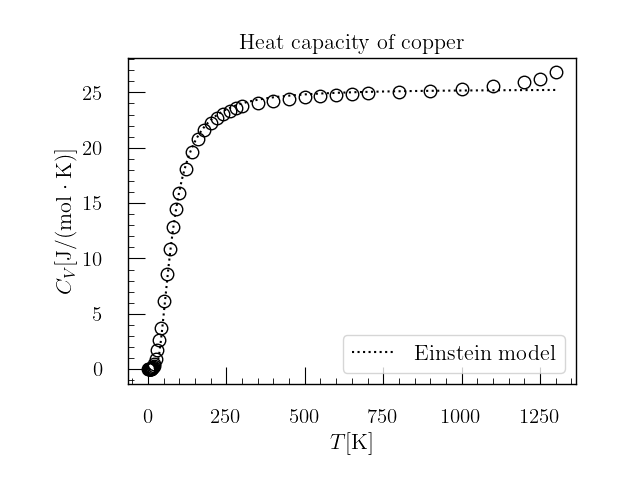
\includegraphics[width=10cm]{./img/einstein_model_copper.png}
			\caption{銅の比熱の実験データとEinstein modelによる結果の比較.銅の比熱のデータは\cite{heat_WC}による.}
			\label{fig:einstein}
	\end{figure}
	非常によくあっているように思える
	\footnote{
			高温でずれるのはなぜだろう.Teamil9さんには銅の融点に近いからその寄与があるのではないか,とご助言いただいた.
	}.実際,高温極限の$3R\sim 25[\mathrm{J/(mol\cdot K)}]$に収束する様子はあっている.ところが,低温の振る舞いは有意に異なって,Einstein modelによるexponentialの収束は実際より強すぎる.実際は$T^3$に比例した振る舞いをする.
	\begin{figure}[H]
			\centering
			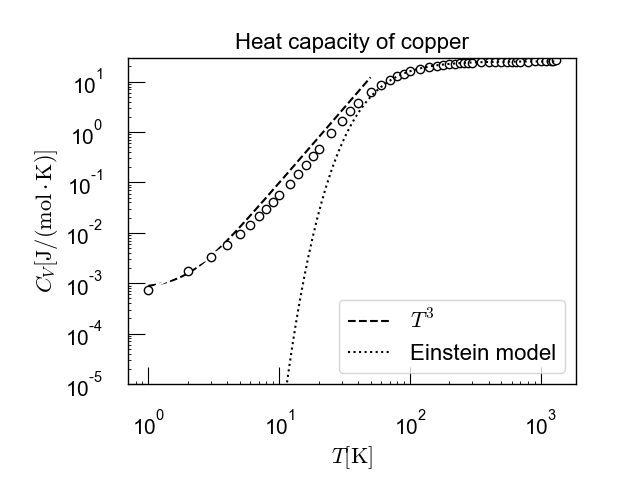
\includegraphics[width=10cm]{./img/einstein_logcompare.png}
			\caption{銅の比熱の実験データとEinstein modelの結果と$T^3$の比較.両対数で見ると,einstein modelによる比熱の関数は振る舞いが明らかに違うことがよくわかる.$T^3$の関数は最初の三点だけfitした.}
			\label{fig:einstein_log}
	\end{figure}
	\subsection{低温での振る舞い}
	低温では比熱は$T^3$に比例した振る舞いをする.これは低温での比熱に寄与する調和振動子の数を調べることでわかる.

	Einstein modelでは調和振動子が独立にあるとして計算したが,実際には粒子間にはもちろん相互作用があり,低温ではその寄与が効いてくるということだ.相互作用を考える場合,粒子同士がバネでつながっている連成振動の問題に帰着される.
	きちんと書くと煩雑になるし,タイプも面倒なので雑な議論をするが,$N$自由度の連成振動自体は位置で議論すると複雑だが,波数で議論すると,波数$k_{\alpha}\in\qty{\pi/ ((L+1)a)n\mid n\in \Z_{>0}}$ごとに調和振動子が一つづつ独立に対応しているものだと思える.ここで,$\alpha$は$x, y, z$の方向をしめすindexである.

	調和振動子が比熱に寄与する,すなわち低温でない条件は
	$k_{\text{B}}T \geq \hbar(\vec{k})$である.
	さらに仮定だが,ほとんどの粒子は$\omega(\vec{k})\sim v_0|\vec{k}|$を満たしているという事実も用いると,
	\begin{align}
			|\vec{k}| \leq k_{\text{B}} T / (v_0\hbar) \label{eq:T3wavelen}
	\end{align}
	を満たす状態の数を勘定すれば良い.

	結果だけ書くと,比熱に寄与する調和振動子の数は,
	\begin{align}
			N(T) \sim \frac{V(k_{\text{B}}T)^3}{6\pi^2 (v_0\hbar)^3}\label{eq:T3statenum}
	\end{align}
	となり,比熱は
	\begin{align}
			c(T) 
			&\sim \frac{3N(T)k_{\text{B}}}{n}\\
			&= \frac{k_{\text{B}}^4 V_0}{2\pi^2 n (v_0\hbar)^3}T^3
	\end{align}
	と大雑把にだが評価される.

	未定義な文字などをたくさんおいているが,重要な$T^3$はEq.\eqref{eq:T3statenum}で状態の数を勘定するとき,条件\eqref{eq:T3wavelen}を満たす半径$|\vec{k}|$の三次元の波数空間の球で評価することにより出現している\footnote{つまり,二次元だと$T^2$に比例するということである.}.以上の議論で,金属の比熱の高温および低温極限での振る舞いが説明できた.

	ところで,中間領域はどうだろう.全領域の比熱の振る舞いを説明する有名なモデルにDebye modelというものがある.これは高温では$3R$に落ち着き,低温では$T^3$で振る舞うというように上の議論を再現する.
	Debye modelによる比熱が中間領域も正確であると言いたいところだが,中間領域の振る舞いは物質に依る.

	結晶構造や,構成粒子の性質など,より精密な構造を反映させたモデルを立てたり,そもそも実際の系で実験することで,中間領域の振る舞いは正確にわかるが,
	そのような詳細な情報がなくても普遍的に金属の比熱には高温,低温での普遍的な振る舞いが宿っていることが物理として面白いと思う.

	\section{理想気体の例}\label{sec:ideal_gas}
	最後に理想気体の状態方程式を導出する.

	
	$N$粒子の自由粒子を考える.これが,理想気体になるという考えである.

	まず,eigen energyを求める. 
	$E_0 = \pi^2 \hbar^2 / (2m)$とおくと,
	\begin{align}
			E = E_0 \sum_{\alpha = 1}^{3}\sum_{j=0}^{N}n_{\alpha, j}^2
	\end{align}
	となる.$\alpha = 1, 2, 3$は$x$, $y$, $z$の方向で,$j$は粒子の番号である.

	次に,分配関数.前につく$1/N!$のfactorは本質でないので特に気にしないでほしいが,
	\begin{align}
			Z(\beta) 
			&= \frac{1}{N!}\sum_{n_{\alpha, j}}e^{-\beta \sum_{\alpha}\sum_{j}n_{\alpha, j}n_{\alpha, j}^2}\\
			&= \frac{1}{N!}\prod_{\alpha}\prod_{j}\sum_{n=1}^{\infty}e^{-\beta E_0 n^2}\\
			&= \frac{1}{N!}\qty(\sum_{n=1}^{\infty}e^{-\beta E_0 n^2})^{3N}
	\end{align}
	と計算できる.ここで和を積分に置き換えるという操作をする
	\footnote{
		この操作は古典極限に対応する.
	}.
	\begin{align}
			\sum_{n=0}^{\infty}e^{-\beta E_0 n^2} 
			&\simeq \frac{1}{\sqrt{\beta E_0}}\int_{0}^{\infty}\dd x e^{-x^2}\\
			&= \frac{m}{2\pi\hbar^2\beta}L
	\end{align}
	であるので,分配関数が
	\begin{align}
			Z(\beta)
			&\sim \frac{V^N}{N!}\qty(\frac{m}{2\pi\hbar^2\beta})^{3N/2}
	\end{align}
	と求まる.ここで$V=L^3$で系の体積である.

	あとは,分配関数を用いて計算するだけで,エネルギーの期待値は
	\begin{align}
			\langle H \rangle &= -\pdv{}{\beta}\log Z(\beta)\\
							  &= \frac{3N}{2\beta}\\
							  &= \frac{3}{2}Nk_{\text{B}}T
	\end{align}
	だし,
	圧力は,Helmholtz free energyの体積微分に負符号をつけたもので,\footnote{引数がめちゃくちゃだが気にしないでくれ.}, Eq.\eqref{eq:Helmholtz}を用いて,
	\begin{align}
			P(\beta, V, N) &= -\pdv{}{V}F(\beta, V, N)\\
						   &= \frac{1}{\beta}\pdv{}{V}\log Z(\beta)\\
						   &=\frac{Nk_{\text{B}}T}{V}
	\end{align}
	と計算でき,$n$をモル数とすると$N=nN_{\text{A}}$,また$k_{\text{B}} = R/N_{\text{A}}$なので,
	\begin{align}
			PV = nRT
	\end{align}
	となる.これは今まで慣れ親しんだ理想気体の状態方程式そのものである.





	\begin{comment}
	\section{canonical分布について}\label{sec:derivation}
	
	対象となる系のeigen energy $E_i$, 体積$V$が大きい熱力学系とエネルギーのやり取りをして平衡状態にあるという状況を考える.
	この大きい熱力学系を熱浴といい, eigen energy $B_i$, 体積$V_{\text{R}}$とする.
	この設定で,対象とする系と熱浴を合わせた全系に対して,等重率の原理を適用することにより,canonical分布を導くことができる.

	起こり得るeigenstateはeigen energyが$U_{\text{tot}} - V_{\text{R}} \delta \leq E_i + B_i \leq U_{\text{tot}} $を満たす状態である.
	やるべきことは,これを満たす状態の数を勘定することである.まず,熱浴についての議論をする.
	満たすべき条件を$\tilde{U}\coloneqq U_{\text{tot}} - E_i $とおくと,

	\begin{align}
			\tilde{U}-V_{\text{R}} - E_i \leq B_i \leq \tilde{U} \label{eq:reserve}
	\end{align}
	となる.熱浴のエネルギー$E$の状態数を$\Omega_\text{R}(E)$とし,
	\begin{align}
			\Omega_i 
			&\coloneqq \Omega_{\text{R}}(\tilde{U}) - \Omega_{\text{R}}(\tilde{U} - V_{\text{R}}\delta)\\
			&= e^{V_{\text{R}}\sigma(\tilde{u}, \rho)} - e^{V_{\text{R}}\sigma(\tilde{u}-\delta, \rho)}
	\end{align}
	は条件Eq.\eqref{eq:reserve}を満たす熱浴の状態の数である.二項の比は
	\begin{align}
			\frac{\Omega_{\text{R}}(\tilde{U}-V_{\text{R}}\delta)}{\Omega_{\text{R}}(\tilde{U})}
			&= e^{-V_{\text{R}}\qty(\pdv*{\sigma{(\tilde{u}, \rho)}}{\tilde{u}})}\\
			&\ll 1
	\end{align}
	となる.最後の評価は熱浴の体積$V_{\text{R}}$が大きいことを用いた.
	結局,
	\end{comment}

\bibliography{booklist}
